\documentclass[10pt,a4paper,twoside,twocolumn]{article}%ustalasz jaki typ dokumentu i właściwości

\usepackage[polish]{babel} % ustawianie języka polskiego
\usepackage[colorlinks=false,linkcolor=green,urlcolor=green,citecolor=green]{hyperref}%hiperłącza ogólnego rodzaju
\hypersetup{pdftitle=Sprawozdanie PSIO}

\usepackage{pdfpages} % importowanie plików z pdfa
\usepackage{amsmath} % do wstawiania macierz itp
\usepackage{graphicx} % wstawianie zdjęć
% \usepackage[utf8]{inputenc} % niepotrzebne bo lualatex
\usepackage[T1]{fontenc} % niepotrzebne bo lualatex
\usepackage[left=2cm,right=2cm,top=2cm,bottom=2cm,
columnsep=1.5cm % odstęp między kolumnami
]{geometry}%marginesy

\usepackage{listings} % punktowanie
% \usepackage{indentfirst} % dawanie akapitu na początku
\usepackage{caption} % podpisy
\usepackage{subcaption} % podpisy do subfigure
\usepackage{siunitx} % jednostki si
\usepackage{minted} % ładne kody naprzyklad matlaba
\setminted{linenos=true,frame=none,breaklines=true,breaksymbolleft=,style=vs,bgcolor={gray!10}}

\usepackage{textcase}

\usepackage[polish,nameinlink]{cleveref} % dobre prefiksy przed etykietą i język
\usepackage{cprotect}

\usepackage{fontspec}
% \setmainfont[Ligatures=TeX]{Georgia}
% \setsansfont[Ligatures=TeX]{Arial}
\usepackage{parskip} % usunięcie tab na początku akapitu
\usepackage{newfloat} % aby można było ładnie wstawić elementy typu zdjecie, kod itp

%%% rysowanie wykresów %%% ale w ciul to trudne więc app.diagrams.net
\usepackage{tikz}
\usetikzlibrary{shapes.geometric, arrows, positioning}

% % % SVG import
\usepackage{svg}
\usepackage{import}
\usepackage{xifthen}
\usepackage{transparent}

% \usepackage{mdframed} % ramki
\usepackage[framemethod=TikZ]{mdframed}
\mdfsetup{%
middlelinecolor=red,
middlelinewidth=1pt,
   backgroundcolor=gray!20,
   roundcorner=10pt}

\usepackage{enumitem} % podpunkty customowe

\usepackage{pgfplots}[compat=1.18] % wykresy

\boldmath%pogrubiona matma

%%%%%%%%%%%%%% koniec pakietów %%%%%%%%%%%%%%%%%%%%%%%%%%%

\title{Fajny ten tytuł}%tytuł
\date{\today}%%data
\author{Janusz Chmaruk}%autor
\setcounter{secnumdepth}{3}%głębokość liczenia roździałów

% PRZYKŁAD LICZNIKA ZADAŃ
\newcounter{zadanie}
\newenvironment{zadanie}[1][]{
   \refstepcounter{zadanie}
   \subsection*{Zadanie \thezadanie#1}
   \addcontentsline{toc}{subsection}{Zadanie \thezadanie#1} % dodanie do spisu treści
}{}

% PRZYKŁAD LICZNIKA ROZWIĄZAŃ
\newcounter{rozwiazanie}
\newenvironment{rozwiazanie}[1][]{
   \refstepcounter{rozwiazanie}
   \subsection*{Rozwiazanie zadania \therozwiazanie#1}
   \addcontentsline{toc}{subsection}{Rozwiazanie zadania \therozwiazanie#1} % dodanie do spisu treści
}{}


% DŁUGIE LISTINGI
\newenvironment{longlisting}{\captionsetup{type=listing}}{}

\newcounter{licznikFigure}
\newcommand{\CC}{\refstepcounter{licznikFigure}\caption*{figure \thelicznikFigure}}


%%%%%%%%%%%%%%%%%%%%%%%%%%%%%%%%%%%%%%%%%%%%%%%%%%%%%%%%%%%%%%%
%%%%%%%%%%%%%%%%%%%%%%%%%%%%%%%%%%%%%%%%%%%%%%%%%%%%%%%%%%%%%%%
%%%%%%% TU SIE ZACZYNA PISANIE PLIKU %%%%%%%%%%%%%%%%%%%%%%%%%%
%%%%%%%%%%%%%%%%%%%%%%%%%%%%%%%%%%%%%%%%%%%%%%%%%%%%%%%%%%%%%%%
%%%%%%%%%%%%%%%%%%%%%%%%%%%%%%%%%%%%%%%%%%%%%%%%%%%%%%%%%%%%%%%

\begin{document}

\null

\includepdf[pages={1}]{Szablon_Projektu.pdf}
\newpage

\tableofcontents
% \newpage

\section{Cel i zakres ćwiczenia}
Celem ćwiczenia jest zapoznanie studentów z działaniem systemu \texttt{roslaunch}.

W ramach ćwiczenia zapoznamy się z:
\begin{itemize}
    \item mapowaniem nazw,
    \item ustawianiem parametrów,
    \item tworzeniem plików \texttt{.launch},
    \item narzędziem \texttt{rosbag}.
\end{itemize}

\section{Przebieg ćwiczenia}
\textbf{Pierwsze zadanie} polegało na tworzeniu wielu węzłów pochodzących z wielu paczek. Tworzenie węzłów służy do skonfigurowania wielu programów oraz ich parametrów. Do procesu uruchamiania stosu ROS jest wykorzystywane narzędzie \texttt{roslaunch}. \texttt{Roslaunch} automatycznie konfiguruje węzły i parametry systemu w oparciu o ustawienia zapisane w plikach XML z rozszerzeniem \texttt{.launch}.

Do tworzenia węzłów można wykorzystać dwa sposoby:
\begin{enumerate}
    \item ręczny, czyli wpisywanie w terminalu,
    \item Pliki \texttt{.launch}, czyli wpisanie plików do konfiguracji zapisywane w formacie XML.
\end{enumerate}

\textbf{Zadanie Układ źródło + regulator + obiekt}

Napisz plik \texttt{.launch} tak, aby utworzyć układ jak na rysunku poniżej. Ustaw parametry węzłów, a następnie pokaż graf systemu (w narzędziu \texttt{rqt\_graph}) oraz przebiegi poszczególnych sygnałów (w narzędziu \texttt{rqt\_plot} lub \texttt{rqt\_gui}). Wypróbuj różne nastawy regulatorów dla wybranych parametrów i typu obiektu (całkujący lub inercjalny) przy zmianie wartości zadanej.

Powyższe zadanie zostało wykonane na dwa sposoby. Pierwszy sposób, ręczne wprowadzenie danych do terminalu.

\begin{figure}[H]
    \centering
    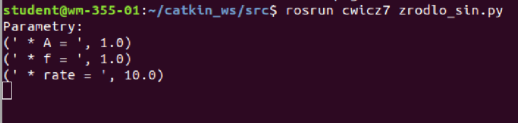
\includegraphics[width=0.9\linewidth]{image1.png}
    \caption{Uruchomienie programu z źródłem}
\end{figure}

Poniżej widać na rys. 2 uruchomienie sumatora gdzie została nadana wartość k2 = -1, aby wykonać sprzężenie zwrotne.

\begin{figure}[H]
    \centering
    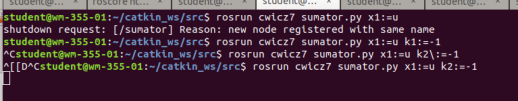
\includegraphics[width=0.9\linewidth]{image2.png}
    \caption{Uruchomienie programu sumator}
\end{figure}

\begin{figure}[H]
    \centering
    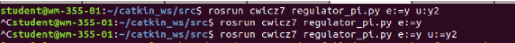
\includegraphics[width=0.9\linewidth]{image3.png}
    \caption{Uruchomienie programu regulatora}
\end{figure}

\begin{figure}[H]
    \centering
    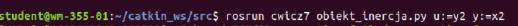
\includegraphics[width=0.9\linewidth]{image4.png}
    \caption{Uruchomienie programu obiektu}
\end{figure}

Następnie został wywołany graf do wyświetlenia węzłów. Na powyższych komendach do uruchamiania programów rys. 2, rys. 3 oraz rys. 4, można zauważyć ustawianie parametrów dla zmiennych wejściowych i wyjściowych. Dzięki temu można utworzyć węzły zobrazowane na grafie rys. 6.

\begin{figure}[H]
    \centering
    
\includegraphics[width=0.9\linewidth]{image5.png}
    \caption{Funkcja do wywołania grafu}
\end{figure}

\begin{figure}[H]
    \centering
    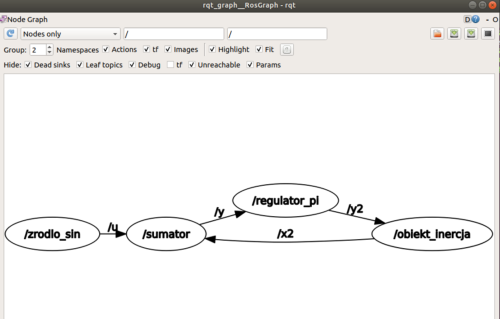
\includegraphics[width=0.9\linewidth]{image6.png}
    \caption{Graf zaimplementowanych elementów}
\end{figure}

Sprawdzenie działania programu oraz wykreślenie przy pomocy programu \texttt{rqt\_plot} wykresu obserwowanych wartości przedstawione jest na rys. 7. Poprzez komendę \texttt{rqt\_plot}.

\begin{figure}[H]
    \centering
    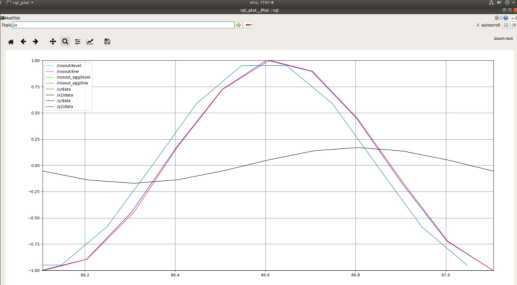
\includegraphics[width=1\linewidth]{image7.png}
    \caption{Wykres działania węzłów}
\end{figure}

Kolejnym etapem było stworzenie pliku \texttt{.launch}, czyli pliku do wpisania konfiguracji węzłów. Tym razem zostało wykorzystane źródło o stałej wartości oraz regulator PID.

\begin{figure}[H]
    \centering
    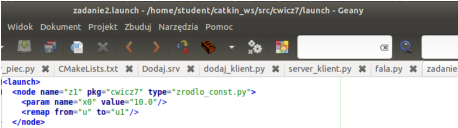
\includegraphics[width=0.9\linewidth]{image8.png}
    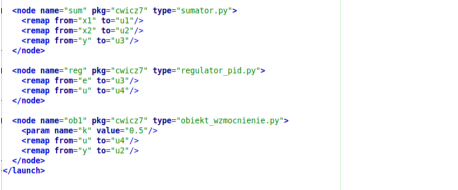
\includegraphics[width=0.9\linewidth]{image9.png}
    \caption{Plik \texttt{.launch}}
\end{figure}

Komendą \texttt{roslaunch} \texttt{miejsce\_zapisu} \texttt{nazwa\_pliku} został uruchomiony plik.

\begin{figure}[H]
    \centering
    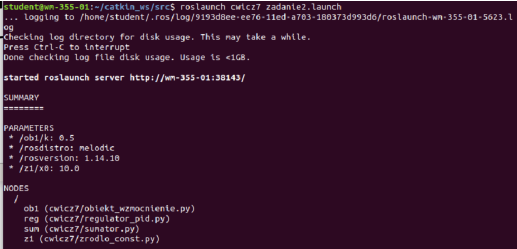
\includegraphics[width=0.9\linewidth]{image10.png}
    \caption{Uruchomienie \texttt{launch}}
\end{figure}

Poniżej na rys. 10 jest przedstawiony graf węzłów. Stworzony z konfiguracją pliku \texttt{launch}.

\begin{figure}[H]
    \centering
    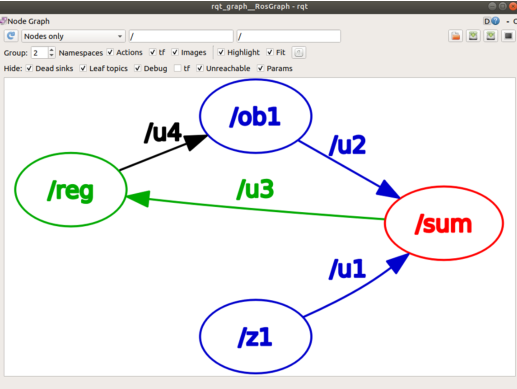
\includegraphics[width=0.9\linewidth]{image11.png}
    \caption{Uruchomienie \texttt{launch}}
\end{figure}

Poniższy wykres jest o stałej wartości, wynika to z zastosowania źródła o stałej wartości.

\begin{figure}[H]
    \centering
    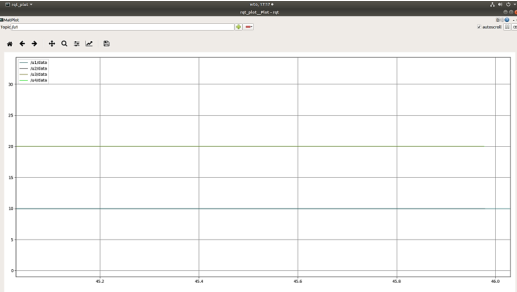
\includegraphics[width=1\linewidth]{image12.png}
    \caption{Uruchomiony wykres działania}
\end{figure}

Zostało również przetestowane inne źródło ramp, czyli sygnał liniowo narastający. Tym razem został wykorzystany regulator PI.

\begin{figure}[H]
    \centering
    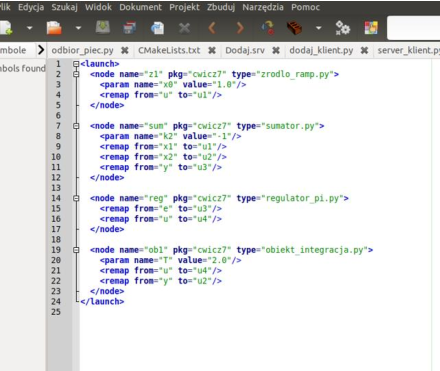
\includegraphics[width=0.9\linewidth]{image13.png}
    \caption{Plik \texttt{.launch} z innymi nastawami}
\end{figure}

\begin{figure}[H]
    \centering
    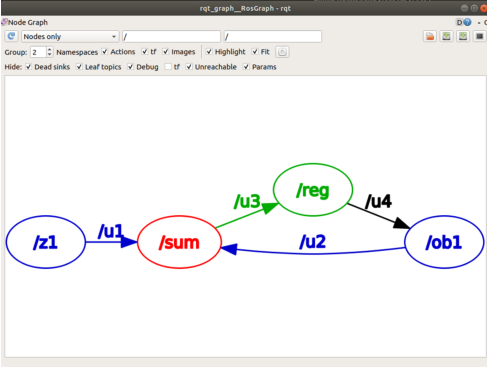
\includegraphics[width=0.9\linewidth]{image14.png}
    \caption{Przedstawiony graf}
\end{figure}

Poniższe wykresy rys. 14 oraz rys. 15 przedstawiają działanie powyższego układu. Można zauważyć, że zmienne wraz z czasem zwiększają swoją wartość.

\begin{figure}[H]
    \centering
    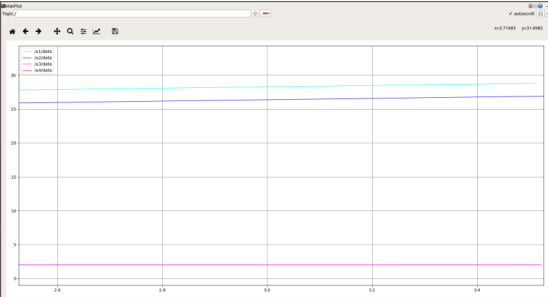
\includegraphics[width=1\linewidth]{image15.png}
    \caption{Przedstawiony wykres w czasie od około 2s do 3,5s}
\end{figure}

\begin{figure}[H]
    \centering
    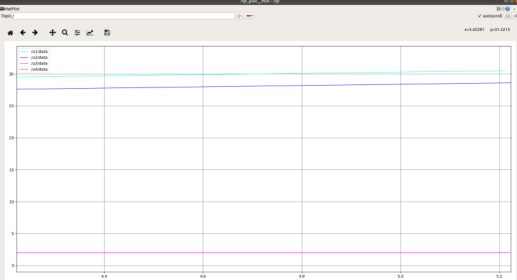
\includegraphics[width=1\linewidth]{image16.png}
    \caption{Przedstawiony wykres w czasie od około 4,2s do 5,2s}
\end{figure}

\section{Wnioski}
Cel ćwiczenia został zrealizowany. Ćwiczenie to pokazuje łączenie kilku programów w jeden układ. Jest to pomocne, kiedy musimy powiązać ze sobą kilka komend w różnych plikach. Istnieją różne możliwości - jedna ręczna z terminala, a druga za pomocą pliku \texttt{launch}. Ten drugi według mnie jest o wiele korzystniejszy ze względu na łatwą możliwość konfiguracji i zamiany danych.

\end{document}
